% textidote: ignore begin
\chapter{Introduction}\label{ch:introduction}
% textidote: ignore end

Chess has seen a rise in player count in recent years, and with the growing player base, the current chess websites have
perfected their craft.
This has been done through intuitive design and the addition of extra features in the apps.
One reason that chess has become more popular online is that using popular web apps like~\url{chess.com} and
\url{lichess.org} allows the player to use chess engines as a powerful tool to aid in their learning journey.

We believe that the utilization of chess engines in the market is not fully saturated yet, as engines are reserved for
single player applications.

% textidote: ignore begin
\begin{figure}[htb]
    \centering
    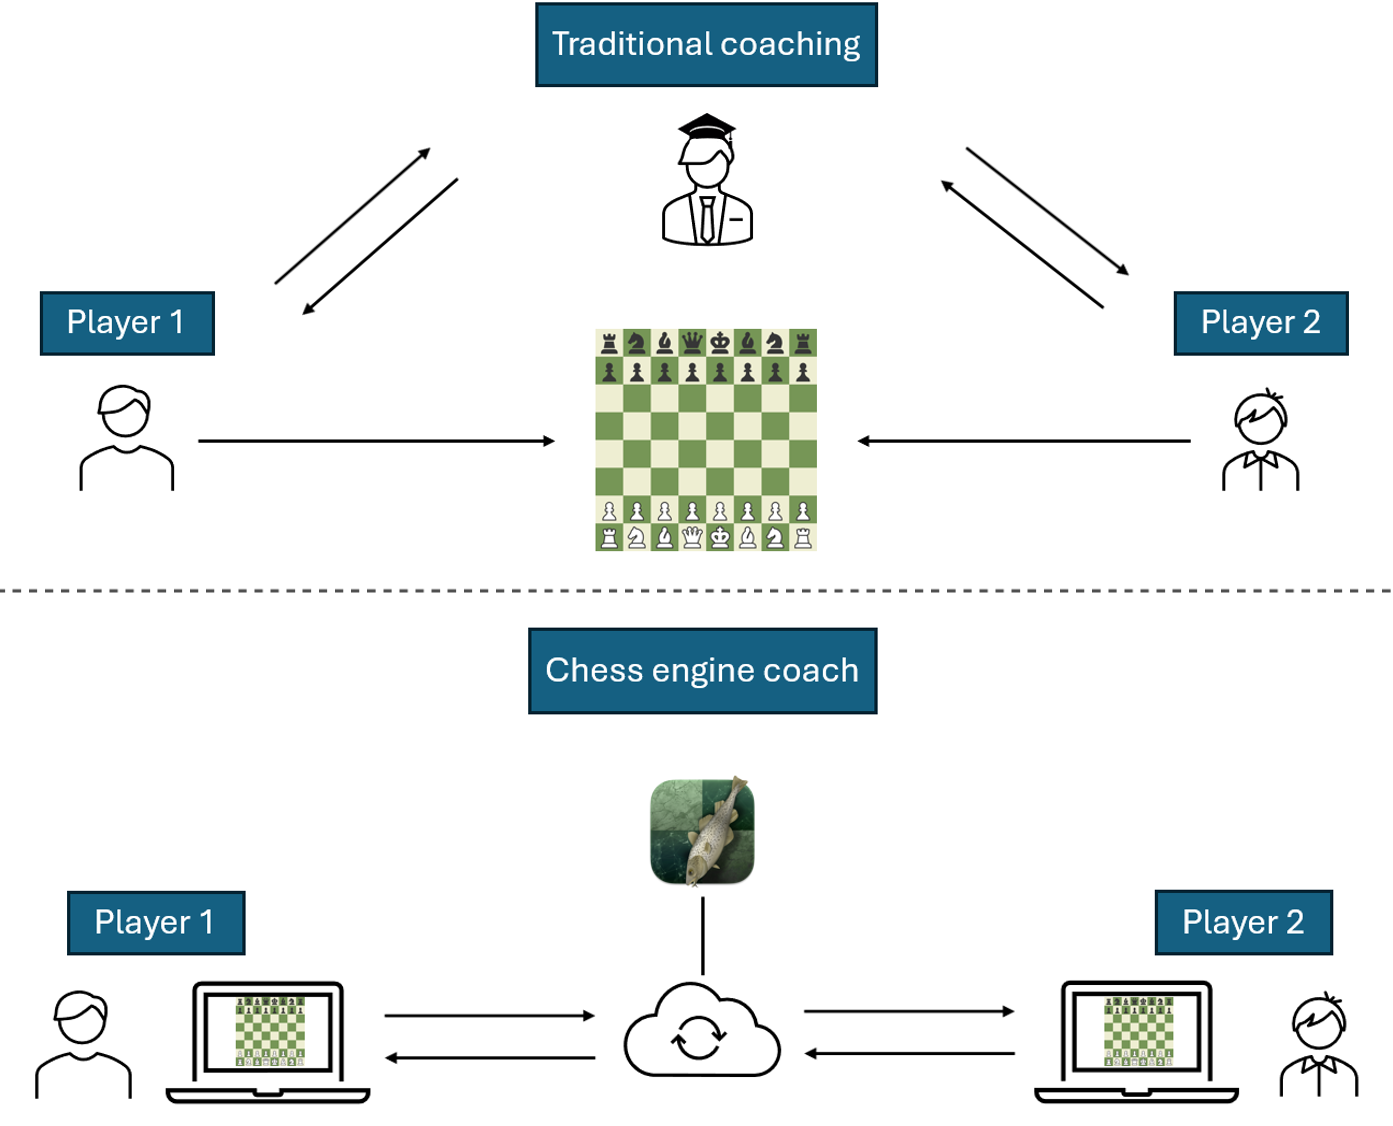
\includegraphics[width=0.7\textwidth]{overview}
    \caption{The two different overall chess learning environments.
    Traditional coaching is a physical coaching session where a coach and some players meet up and play over the board.
    Chess engine coaching exists online in the cloud, why no physical meeting is necessary.}\label{fig:project-overview}
\end{figure}
% textidote: ignore end

Chess engine popularity has risen greatly in the past years and has been developed to a point that they
outperform humans.
These tools are essential for understanding the complex mid- and endgame strategies of chess.
This makes engines an optimal tool for teaching players the intricacies of chess, which is what
differentiates the average chess players from masters.

Chess encapsulates the spirit of a game that is easy to learn, but hard to master.
That is why those who wish to become skilled in chess seek help from other masters in the form of a coach.
Coaching is a well-respected form of learning, but it has flaws that place barriers in terms of who can get this form of
help.

The biggest obstacle coaches have is the monetary aspect as most players do not have the money to afford a chess coach
for extended periods of time.
Coaches also need to have allocated time for their lessons, which means that it makes it more difficult to have the
coaching sessions.

We will be focusing on the learning aspect of chess by making a chess web app that allows two players to play against
each other with a coach.
This coach will be a chess engine, which will allow both players to learn while playing in a multiplayer environment, as
seen in Figure~\ref{fig:project-overview}.

The authors have given this project the name ChessTeacher, which encapsulates the goal of the project, while being
short and concise.

Through this approach, we touch a niche that lies between the social aspect of a player vs.\ player chess game and the
great learning tools that are made to study chess and its complexities individually.
The product we are suggesting will implement the best from both worlds by targeting the social aspects of the game while
still providing useful information to the player on how to improve their chess capabilities.
By making use of engines and online services, we can also address the time and monetary problems of coaching.
